\documentclass[twocolumn]{article}
\usepackage{amsmath}
\usepackage{caption}
\usepackage{graphicx}
\usepackage{yfonts}
\usepackage{listings}
\usepackage{lipsum}
\usepackage{multicol}
\usepackage{hyperref}
\usepackage{color}
\usepackage{wrapfig}

	\title{PHYS488: Week5 - Group Tasks introduction}
	\author{Luke Jones, Lorna Baker, Zachary Humphreys}	
	\lstdefinestyle{custom}{basicstyle=\tiny,language=java,showspaces=false,showstringspaces=ffalse,tabsize=1,keepspaces=true}
	\lstset{style=custom}

\begin{document}
	
\maketitle
\begin{abstract}
	\begin{center}
		\textit{This weeks work introduced the aspect of group work as a lead-up to the projects, whilst expanding on the knowledge of simulations. In Task 1, two reusable classes were made that do simple calculations for Muons passing through a material that can be used as an object within executable code to find both their energy loss, and Coulombic scattering. In Task 2, a much larger simulation was done, again using these classes to produce trajectories and energy distributions through muons passing through a simulated material to several detectors.}
	\end{center}
\end{abstract}	
%Main Body of text in 2Column format

\section{Task 1}
For this task we were tasked with creating 2 classes called \textbf{EnergyLoss} and \textbf{MCS}. The first part was to create a class to calculate energy loss from material and particle parameters, the \textbf{EnergyLoss} class, with the second to create a class to work out the multiple coulomb scattering, \textbf{MCS}.\\\indent This task is designed so that for the instantiation the parameters that are typed in are the only the variables needed to work out the energy loss. The parameters are the: atomic mass, atomic number, and the density of the material. To work out the energy loss the following 2 equations have to be used which are listed equation 1 and 2 where $K$ is a constant equal to $0.07075 MeVcm^{-1}$, $m_{e}$ is the electron rest mass equal to $0.511 MeV$, $I$ is the mean excitation energy equal to $0.0000135*Z MeV$, and as the task was working with muons, $z$ is the muon charge equal to $1$, and $M$ the rest mass equal to $106 MeV$.
	\begin{align}
	W_{max}&=\dfrac{2m_e \beta^2 \gamma^2}{1+(2 \gamma m_e)/M+(m_e/M)^2}     \\
	\langle\dfrac{dE}{dx}\rangle &= Kz^2 \rho \dfrac{Z}{A}  \dfrac{1}{\beta^2} [\dfrac{1}{2} ln(\dfrac{2m_e \beta^2 \gamma^2 W_{max}}{I^2})] 
	\end{align}
Using these 2 equations and the parameters which were given on the task sheet, the only parts that need to be worked out are beta and gamma which are both relativistic variables. The equation listed as equation 3 works out the energy of the muon ($E$) which is needed for equation 4 which works out beta(the speed of the particle as a fraction of the speed of light). Equation 5 uses beta to work out Lorentz factor, where P is the momentum of the muon. All other symbols retain their previous meaning.
	\begin{align}
	E &= \sqrt{M^2 + P^2} \\
	\beta &= \dfrac{P}{E} \\
	\gamma &= \dfrac{1}{\sqrt{1-\beta^2}}
	\end{align}
\\ \indent A class file was made which was very similar to the \textit{Histogram.java} in terms of structure used in the previous weeks. The class is called \textbf{EnergyLoss} and the contents first states all the variables used and then has a constructor for the class which is where the parameters go into. Inside the constructor contain code specifying the input values for that instance of the class. After this, a method was made called \textit{getEnergyLoss} which, when the momentum of the muon is inserted, returns the energy loss calculated using the parameters. This method has all the equations needed to work out the energy loss inside it. The code for the class may be found in Appendix A. \footnote[1]{All the code for this weeks tasks can be found \url{https://github.com/donmegamuffin/Phys488_Workshop5/tree/master/Programs/BlueJ}}
\\ \indent The second part of this task was to create a program to calculate the multiple coulomb scattering (MCS) of a particle moving through a material. This required the creation of a program similar in style to the previous part, a separate class with a constructor to be used as an object within an executable program. It had three methods, each to solve one of the following equations: 
	\begin{align}
	X_0 &\approx \dfrac{716.4A}{\rho Z(Z+1)  \ln{(\frac{287}{\sqrt{Z}})}} \\ 
	\theta_0 &= \dfrac{13.6 MeV}{\beta P}z\sqrt{\frac{x}{X_0}} \\
	\theta_t &= \sqrt{2}\theta_0
	\end{align}
where $X_0$ is a radiation length, $\rho$ is the density of the material, and the other variables retain their previous meanings. \\ \indent It was requested the constructor for object take in the parameters of the material ($Z,A,\rho$) as arguments to construct an MCS object, and that the methods take in the particle's momentum and the material's thickness as arguments. As the task only required calculations for muons, the particle mass and charge as well as the Rydberg constant were stored globally using the \textit{private final} modifiers. This meant they could not be altered from outside the program or by the program itself. The other variables for the material were also global, but initialised without values to then be given values once instantiated by an executable through the constructor. \\ \indent The first of the three methods was the \textit{getX\_0} method which simply calculated the radiation length and returned it requiring no parameters outside of those initialised by the constructor. \\\indent The second method calculated the $\theta_0$ of the system called \textit{getTheta0} and required the momentum and thickness arguments. As it required the value of $X_0$, it would first do a calculation which called the \textit{getX\_0} method, then proceed with the rest of the calculation, returning the value $\theta_0$. \\\indent The last method was the calculation of the $\theta_t$ value which itself was a simple calculation but required $\theta_0$ which itself required the momentum and thickness arguments, so this method too required them, and would simply parse them to the \textit{getTheta0} method's arguments. This method was called \textit{getThetaT} in line with the rest of the naming scheme. The code can be found in Appendix B.
\\\\indent The last part of this task was to then write a program to simply initialise the previous two classes within an executable program and test them with a series of momenta values to check if the programs were functioning correctly. To do this, the momenta values wanted for the task were stored as 2 arrays of \textinit{double[]}, one for the calculation of $\dfrac{dE}{dx}$ with the energy loss program, and a second set for the calculation of $\theta_t$ using the MCS program. This saved on many lines of code and prevented needing many different variables, or having them programmed directly in as magic numbers. As well as that, another benefit is that they array can be altered or added to at any time, accessed easily from right at the top of the program. \\\indent The next 2 lines initialised MCS and EnergyLoss as objects with the parameters for Iron as requested, and one more global variable was added which was the thickness of the iron, as this was set by the task and did not require altering and thus having it as a global variable allowed it to be changed easily and accessibly at the top of the file rather than baking it directly into the code as a magic number. \\\indent The main method has two main parts, reflecting that of the target console output for the task. These were two loops that would cycle through the array values until it hit the end of the array by using an $n<array.length$ parameter for the \textinit{for} loop.
\begin{table*}[h]
	\hrule
	\begin{lstlisting}	
																									The values for energy loss: 
																									dE/dx = 81.52 MeV/cm for p = 30.0 MeV
																									dE/dx = 11.59 MeV/cm for p = 300.0 MeV
																									dE/dx = 15.26 MeV/cm for p = 3000.0 MeV
																									dE/dx = 17.72 MeV/cm for p = 10000.0 MeV
																									dE/dx = 19.81 MeV/cm for p = 30000.0 MeV
																									dE/dx = 21.96 MeV/cm for p = 100000.0 MeV
																									
																									The values for MCS:
																									Iron X0 = 1.797cm
																									For a material thickness of 1cm:
																									thetaT = 0.02868 for p = 500.0 MeV
																									thetaT = 0.01411 for p = 1000.0 MeV
																									thetaT = 0.00468 for p = 3000.0 MeV
	\end{lstlisting}
	\caption{\label{tab:Task1} This is the text output from console for Task 1.}
	\hrule
\end{table*} \\\indent Often, to maintain the same number of significant figures as the requested output, the \textit{printf} function had to be used coupled with $\%.xf$ where $x$ was the number of decimal places needed. The program could have been written in approximately half the lines of code without this, so a more general solution for printing correct significant figures within a \textit{println} command will need to be found in future, as \textit{println} can output many things, but \textit{printf} appears to be limited to one string and a variable if using the $\%.xf$ command. The output of this code was can be found in Table \ref{fig:Task1}.

Note, for the thetaT outputs, the first two have an addition significant figure over the requested as for $p = 3000MeV$ it required an additional significant figure, and so the entire looped was set to that. The code is found in Appendix C.

\section{Task 2}
This part of the tasks involved the investigation of tracking a muon travelling through an iron sheet, whereby the simulation of such a particle is monitored by counting the ‘hits’ on two detectors placed at 10cm and 20cm beyond the back of the iron. The code \textbf{TrackMuon} was downloaded from VITAL and put into BlueJ, whereby several adjustments were made in order to carry out the assigned tasks. \\\indent First it was necessary to ensure an understanding of how the program itself operated. By input of the necessary code, the instance classes for \textbf{Energy Loss} and \textbf{MCS angle} (previously created in Task 1) were added to the \textbf{TrackMuon} code, in order to calculate both these aspects through each step of the detector. The energy loss was taken into account by taking away the energy loss at each step by multiplying by the distance it had taken, which in this case is \textit{d}. While the MSC angle was taken into account by changing theta to $\theta$ plus a Gaussian with a mean of 0 and a width of the MSC angle $\theta_t$. It should be noted that the constructor for the energy loss was put in normally while the constructor for the MSC angle had to be put within the loop because the thickness changed at each step so the thickness should be the variable step. \\\indent From the assumption that the muon starts at position co-ordinates $(x, y) = (0, 0)$, i.e. just inside the iron, the user is prompted to type in the initial variables that will be used within the program, including: starting energy, step size, thickness of the iron and the number of muons to track. The positions of the aforementioned counters that detect the muons are also defined in the code. \\\indent Muons are tracked through the iron in small steps (whose size is specified by the user), and the energy loss and MCS angle is calculated at each of these steps. As the particle is followed, the $(x, y)$ position co-ordinate pairs are stored in a 2D array (\textit{trackOfMuon}). This array was developed via use of a \textit{for} loop that laid out the initial \textit{double} values that were to be measured, inclusive of the start energy, the initial starting position (for both x and y co-ordinates), the number of steps and the angle at which the muon starts out (parallel to the x-axis). A \textit{while} loop within this then stores each step and the scattering angle, as well as also incorporating a \textit{nextGaussian} instruction to return randomly generated values of $\theta$ around the mean of the distribution. \\\indent The use of an \textit{if} loop was also used to cause a break in the \textit{for} loop should either the energy of the muon fall below the rest mass. The maximum value of steps that the muon was to be tracked for was set to 200. The muons will be tracked at each step and will be followed until the use of a second \textit{if} loop causes another \textit{break} should the number of steps taken by the muon go above this set value nmax. Thus, overall the muon is tracked until either of the two specified \textit{if} loops are enabled, or until the muon leaves the back of the iron sheet. Should the tracking of the muon fall within the allowed parameters and pass through the back of the sheet, the co-ordinate values are then stored in the double array for each point through the detector. \\\indent Upon completion of this array, the useful information is then passed to the class method \textit{lookAtThisMuon} in order to be prepared for external analysis.   In order to export data from the program, the \textit{writeToDisk} function was also included to enable data to be exported as .csv file for analysis in Excel. \\\indent First it was required that the co-ordinates of 10 sample muon tracks (the (x, y) pairs) were written to a file on disk and plotted as a scatter chart in Excel and can be seen in Figure \ref{graph1}.
\begin{figure}[h]
	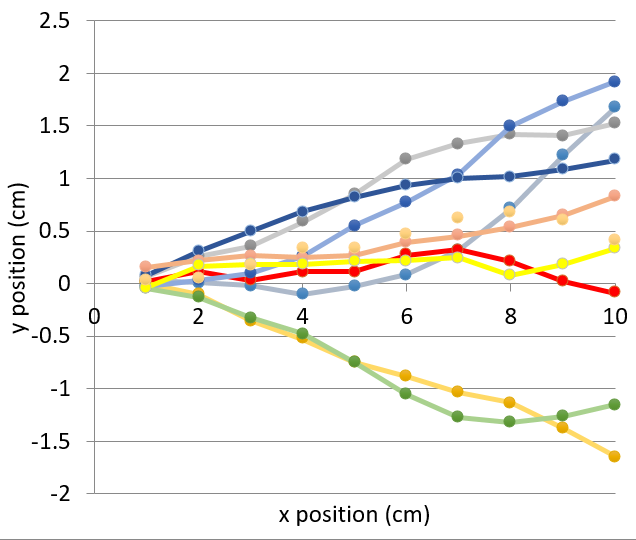
\includegraphics[scale=0.3]{Images/Graph1.png}
	\caption{\label{graph1}Scatter graph depicting the x and y co-ordinate pairs of 10 sample muon tracks travelling through the first 10cm of the iron sheet.}
\end{figure}
From this plot is may be observed that each of the muons follow a similar path through the first 2-3cm of the iron. After a few centimetres however, it may be seen that due to the addition of further MSC angles through each step, there is a greater effect on the y-position of each muon - thus their paths begin to spread further from each other and change track as they travel along the x-axis. \\\indent Further code was also required in order to generate histogram plots of the exit energy and y-positions of the muons as they exit the back of the iron sheet. This was done by first adding 2 array, \textit{ylastE} and \textit{muonenergyXY}. The first array \textit{ylastE} was set so for each loop it will add in the y position as it leaves the iron, while the \textit{muonenergyXY} does the same for the energy. Both of these are found the same was as it is found in \textit{lookAtThisMuon}. The next step was to be able to plot it, to do this a new \textit{WriteToDisk} function was made, this one being called \textit{WriteToDiskXY}. This new function had the inputs of both arrays, nsteps, and the filename instead of just the filename. The inside of the function was the same expect the only output files were the 2 arrays and position which were in the loop. \\\indent The output energy and y position were calculated with a step value of 1 cm and a thickness of 1 cm with 10,000 muons. While the energy was first at 10,000 MeV, then at 5,000 MeV, and then at 500 MeV. This was done for 3 different energies to see the difference between them so comparisons can be made. The first graph which was made using the 10,000 MeV energy can be seen below under Figure \ref{graph2}, while Figure \ref{graph3} represents the 5,000 MeV energy graph, and Figure \ref{graph4} represents the 500 MeV energy graph. The 500 MeV graph has 97 muons which have stopped inside the iron, while the rest made it out of the iron. 
\begin{figure}
	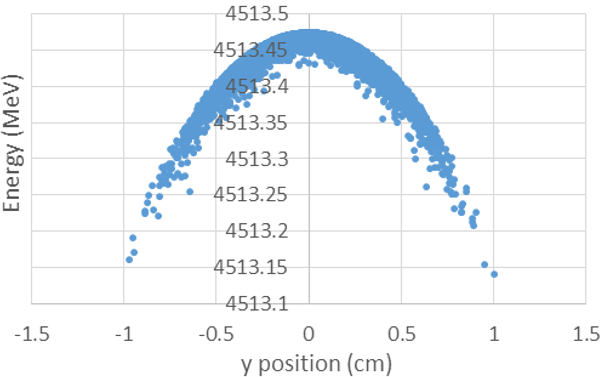
\includegraphics[scale=0.3]{Images/Graph3.png}
	\caption{\label{graph2}Graph showing the energy of a muon at it leaves the iron and also the y position that the muon left at. This is for a starting energy of 10,000 MeV.}
\end{figure}
\begin{figure}
	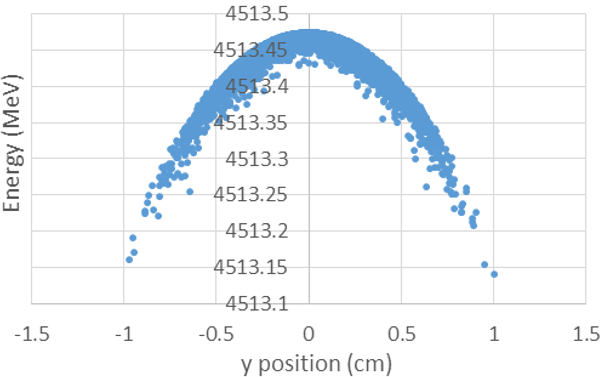
\includegraphics[scale=0.3]{Images/Graph3.png}
	\caption{\label{graph3}Graph showing the energy of a muon at it leaves the iron and also the y position that the muon left at. This is for a starting energy of 5,000 MeV.}
\end{figure}
\begin{figure}
	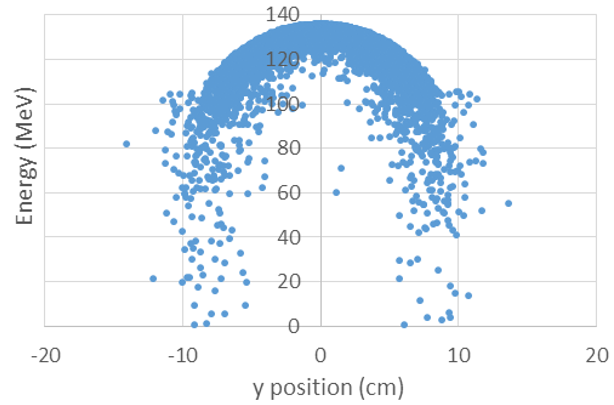
\includegraphics[scale=0.3]{Images/Graph4.png}
	\caption{\label{graph4}Graph showing the energy of a muon at it leaves the iron and also the y position that the muon left at. This is for a starting energy of 500 MeV.}
\end{figure}

\indent It can be seen from looking at Figure 2, 3, and 4 how different starting energies affect the energy that it leaves the iron at. As the starting energy decreased the range of the y position increased also, this is because there are many more collisions when the muons are going slower. It can also be seen how as the starting energy decreases, the energy gap between highest and the lowest energy muon leaving the iron increases. This energy gap is greatest as the energy is very low and can be seen to be of around 140 MeV. It can also be seen that at the very low starting energy the distribution becomes a lot more wide and scattered, this is due to the amount of random collisions occurring.\\\indent The next task asks to add in another detector this time 30 cm away from the iron and to plot histograms for each detector. This was done by adding in another contractor this time called \textit{detector3}. Then another xc3 to determine the distance the detector is away, then adding another \textit{yhitOnC3}, then another \textit{trackOfMuon}, then filling the histogram, and finally writing the histogram to disk. All these steps are very similar to what is done for detector 2 compared to detector 1. Once the third detector was added the program was run with an energy of 1,000 MeV, steps of 1 cm, thickness of 30 cm, and 10,000 muons. The bin high and bin low of all three detector was set to ± 15. Figure 5, 6, and 7 show each detector where Figure 5 is for detector 1, Figure 6 for detector 2, and Figure 7 for detector 3.
\begin{figure}
	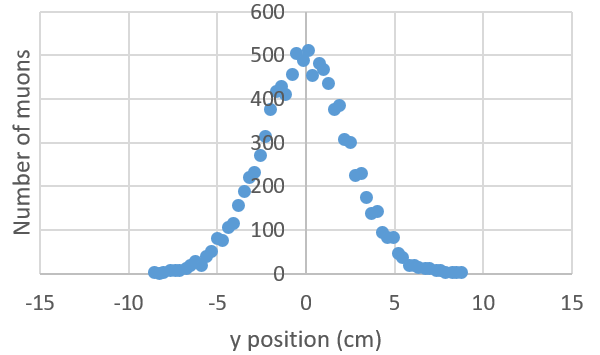
\includegraphics[scale=0.3]{Images/Graph5.png}
	\caption{\label{graph5}Graph showing the number of muons vs the y positions for detector 1.}
\end{figure}
\begin{figure}
	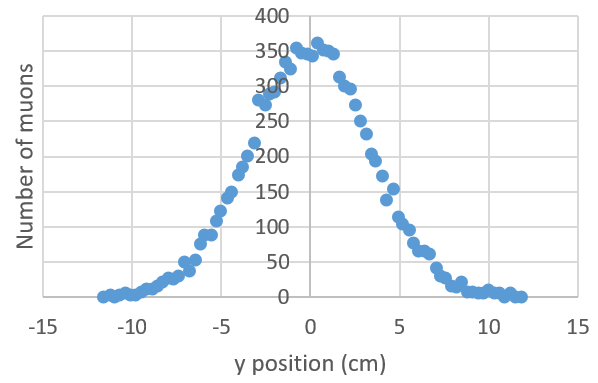
\includegraphics[scale=0.3]{Images/Graph6.png}
	\caption{\label{graph6}Graph showing the number of muons vs the y positions for detector 2.}
\end{figure}
\begin{figure}
	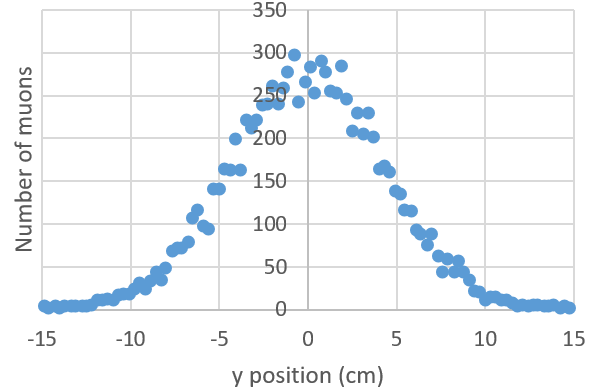
\includegraphics[scale=0.3]{Images/Graph7.png}
	\caption{\label{graph7}Graph showing the number of muons vs the y positions for detector 3.}
\end{figure}
\indent It can be seen from looking at the 3 graphs that the further away the detectors the more spread out the muons are, this is what is expected because of the angle of the muons emerging from the iron. This is because when the muons emerge with an angle the further away they go the further from the midpoint they will go. 

\section{Distribution of work}
Zachary Humphreys: wrote the \textbf{MCS} and \textbf{Task1} code, and cleaned and commented \textbf{EnergyLoss}. He wrote his section on MCS and Task 1 (second half of task 1 in the report). He compiled the other report submissions into \LaTeX.

\appendix
\onecolumn
\scriptsize
NOTE: Task code can be found online at \url{https://github.com/donmegamuffin/Phys488_Workshop5/tree/master/Programs/BlueJ} for easier reading.
\section{Task1: Energy Loss Code}
\begin{verbatim}
/*  Authors: Luke Jones, Zachary Humphreys, Lorna Baker
*   Intructions: 
*   2 Sets of inputs are required for all of the code to function.
*   1)The constructor requires 3 material arguments (in order): atomic number, atomic mass, density.
*   2)The getEnergyLoss method require addition arguments: particle momentum (MeV), and material thickness (cm)
*/

import java.io.*;

class EnergyLoss
{   
	//Universal constant
	private final double K = 0.307075;          // MeV cm^2
	private final double electronmass = 0.511;  // MeV
	private final double c = 3E8;               // m/s     
	//Material variables
	int AtomicNumber;           // atomic Z
	double AtomicMass;          // atomic A
	double density;             // of material
	//Particle variables
	double charge = 1;          //Coulombs
	double mass = 106;          // MeV
	
	public EnergyLoss(int Z, double A, double p) 
	{
		AtomicNumber = Z;
		AtomicMass = A;
		density = p;       
	}
	
	public double getEnergyLoss(double m)
	{
		double momentum = m;                                                       //MeV
		double energy = Math.pow((Math.pow(momentum,2)+Math.pow(mass,2)),0.5);     //energy of muon //MeV      
		double Beta2 = Math.pow((momentum/energy),2);                              //Velocity as fraction of speed of light squared
		double Gamma2 = Math.pow((1/(Math.pow((1-Beta2),0.5))),2);                 //Lorentz Factor squared
		double I = 0.0000135*AtomicNumber;                                         //Mean excitation energy //MeV
		double Wmax = (2*electronmass*Beta2*Gamma2)/(1+((2*Math.sqrt(Gamma2)*electronmass)/mass)+Math.pow((electronmass/mass),2));
		double energyloss = K*Math.pow(charge,2)*density*(AtomicNumber/AtomicMass)*(1/Beta2)*(0.5*Math.log((2*electronmass*Beta2*Gamma2*Wmax)/Math.pow(I,2))-Beta2);
		
		return energyloss;          // energy lost per distance (MeV/cm
	}    
}


\end{verbatim}
\section{Task1: MCS Code}
\begin{verbatim}
/*  Author: Zachary Humphreys; ID:200951438
*   Intructions: 
*   2 Sets of inputs are required for all of the code to function.
*   1)The constructor requires 3 material arguments (in order): atomic number, atomic mass, density.
*   2)The theta methods require addition arguments: particle momentum (MeV), and material thickness (cm)
*/
import java.io.*;

class MCS
{
	// Stating Global variables needed for class
	//Constants
	static private final double Rydberg_constant = 13.6;    //MeV
	//Material properties
	private double material_density;                        //gcm^{-3}
	private int    material_Z;
	private double material_A;
	//Particle variables: Taken as constants
	private final double particle_charge = 1;                     //Coulombs
	private final double particle_mass = 106;                     //MeV
	
	//Constructor
	public MCS(int in_Z, double in_A, double in_density)
	{
		material_density = in_density;
		material_Z = in_Z;
		material_A = in_A;
	}
	
	//Calculates the material radiation length
	public double getX_0()
	{
		double X_0 = ((716.4*material_A)/(material_density*material_Z*(material_Z+1)*Math.log(287/Math.sqrt(material_Z))));
		return X_0;
	}
	
	//Calculates the theta_0 angle of scattering
	public double getTheta0(double particle_momentum, double material_thickness)
	{
		double x_ratio = material_thickness/getX_0();
		//Calculates the velocity as speed of light fractions
		double particle_beta = (particle_momentum/Math.sqrt((Math.pow(particle_momentum,2)+Math.pow(particle_mass,2))));
		double theta_0 = ((Rydberg_constant*particle_charge*Math.sqrt(x_ratio))*(1+0.038*Math.log(x_ratio))/(particle_beta*particle_momentum));
		return theta_0;
	}
	
	//Calculates the theta_t angle of scattering
	public double getThetaT(double particle_momentum, double material_thickness)
	{
		double theta_t = (Math.sqrt(2)*getTheta0(particle_momentum, material_thickness));
		return theta_t;
	}
}
\end{verbatim}
\section{Task1: Executable Code}
\begin{verbatim}
/* Author: Zachary Humphreys; ID:200951438
*   Intructions: 
*   Please input the momentum energies you require into the array lists p1/p2 that you want to console
*   NOTE: This has only the outputs and properties for IRON baked in (COPPER properties commented out; print code omitted).
*/
import java.io.*;

class Task1
{   //Data values for task question part 1, and part 2
	static double[] p1_array = {30,300,3000,10000,30000,100000};   //stores part1 momenta
	static double[] p2_array = {500,1000,3000};                    //stores part2 momenta
	//Initialise Materials IRON:
	static EnergyLoss ironEloss = new EnergyLoss(26,55.845,7.87);
	static MCS ironMS = new MCS(26,55.845,7.87);
	static final double iron_thickness = 1;                        //cm
	/*COPPER:
	EnergyLoss copperEloss = new EnergyLoss(29,63.546,8.96);
	MCS copperMS = new MCS(29,63.546,8.96);
	*/
	public static void main()
	{
		System.out.println("\nThe values for energy loss:");
		//Cycles through until it reaches the end of the array of momenta values
		for(int n=0;n<p1_array.length;n++)
		{   //This prints out the output wanted from part 1 cycling through the array values to console
			System.out.printf("dE/dx = %.2f",ironEloss.getEnergyLoss(p1_array[n])); //For 2 decimal points
			System.out.println(" MeV/cm for p = "+p1_array[n]+" MeV");
		}
		System.out.println("\nThe values for MCS:");
		System.out.printf("Iron X0 = %.3f",ironMS.getX_0());
		System.out.println("cm\nFor a material thickness of 1cm:");
		for(int n=0;n<p2_array.length;n++)
		{   //This prints out the output wanted from part 2 cycling through the array values to console (5 sigfig)
			System.out.printf("thetaT = %.5f",ironMS.getThetaT(p2_array[n],iron_thickness));
			System.out.println(" for p = "+p2_array[n]+" MeV");
		}
	}   
}
\end{verbatim}
\end{document}
